\section{Experiments and Results}

\begin{table*}
\renewcommand{\arraystretch}{1.3}
\centering
\caption{Performance of the networks on the Tobacco-3482 dataset with $100$ training samples per class and different weight initializations.}
\begin{tabular}{l|c|c|c}
 & Document Pretraining & ImageNet Pretraining & No Pretraining \\\hline
AlexNet & $90.04\,\%$ & $75.73\,\%$ & $62.49\,\%$ \\\hline
GoogLeNet & $88.40\,\%$ & $72.98\,\%$ & $70.28\,\%$ \\\hline
VGG-16 & $91.01\,\%$ & $77.52\,\%$ & $69.50\,\%$ \\\hline
Resnet-50 & $91.13\,\%$ & $67.93\,\%$ & $59.55\,\%$
\end{tabular}
\label{tab:accuracy_small}
\end{table*}



\subsection{Datasets}
To evaluate the performance of the deep neural networks presented in section \ref{sec:networks}, two datasets are used. First, we train a variety of networks on the Ryerson Vision Lab Complex Document Information Processing (RVL-CDIP) dataset \cite{harley2015evaluation}. This dataset consists of $400,000$ labeled document images from 16 classes. The dataset is already split into a training dataset which contains $320,000$ images and a validation and a test dataset which each contain $40,000$ images.

Secondly, we use the Tobacco-3482 dataset \cite{doclass_Kumar14} to evaluate the performance of the deep \ac{cnn}s and to investigate to which extent transfer learning from the first dataset is applicable. The Tobacco-3482 dataset contains $3,482$ images from ten document classes. 

Both datasets are quite similar and there even exists some overlap. Therefore, at the transfer learning experiments, we pretrain the networks not on the full RVL-CDIP dataset, but only on the images that are not contained in the Tobacco-3482 dataset. Thus, the networks are pretrained on only $319,784$ training images.




\subsection{Evaluation}

For the RVL-CDIP dataset, we just train the networks and report the top-1 accuracy achieved on the test set. Since the Tobacco-3482 dataset is so small, we use a slightly more sophisticated evaluation technique to get an expected accuracy and to avoid unrepresentative results due to random initialization or a specific dataset split. To come up with a robust estimate of how well the networks perform, we split the dataset such, that $10$ to $100$ images per class are used for training while the rest are for testing. The training dataset is again split with an $80/20$ ratio, so that $20\,\%$ of the training data are used for validation. For each split size, we randomly create ten dataset partitions and report the median accuracy achieved by the networks.
This is similar to the evaluation scheme that was also used by Kang et al.~\cite{lekang_14_a} and Kumar et al.~\cite{doclass_Kumar14} and allows for a fair comparison with their approaches.


\subsection{Results on Tobacco-3482}

\begin{figure}
        \centering
        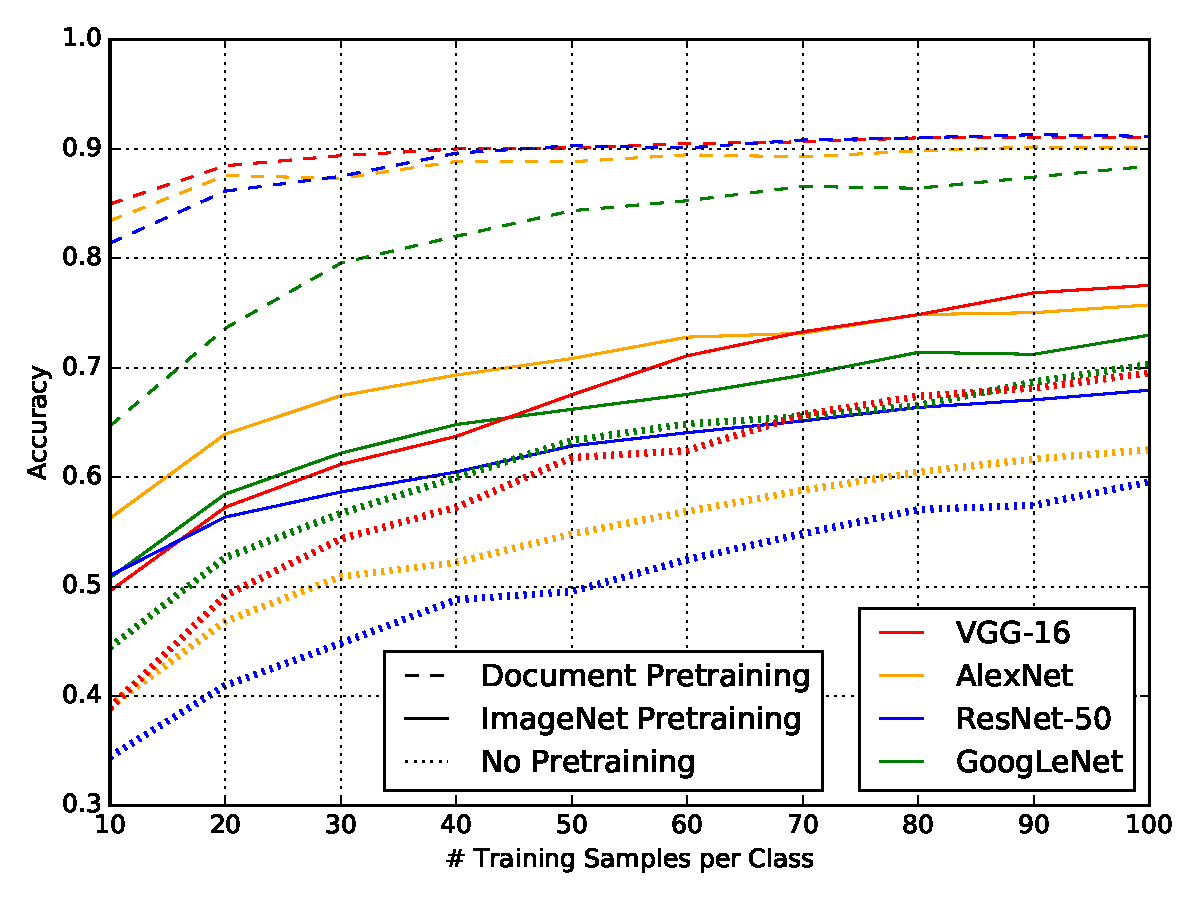
\includegraphics[width=\linewidth]{accuracy_compare.pdf}
        \caption{Mean accuracy achieved on the Tobacco-3482 dataset. The dashed graphs represent the networks that are pretrained on the RVL-CDIP dataset, the solid lines represent the network with ImageNet pretraining and the dotted lines show the network accuracy when trained from scratch.}
\label{fig:accuracy}
\end{figure}



We have trained the four deep \ac{cnn}s described in Section~\ref{sec:networks} on the two datasets with different weight initializations to investigate the benefits of transfer learning. As shown in Table~\ref{tab:accuracy_small} and Fig.~\ref{fig:accuracy} which correspond to the achieved performance on the Tobacco-3482 dataset, transfer learning does improve the classification performance significantly. When the networks are pretrained on a similar dataset, the accuracy achieved on the final dataset is higher than $90\,\%$ and already with as little training data as $10$ samples per class, we could outperform the current \sota which achieves only $77.6\,\%$~\cite{afzal2015deepdocclassifier}.


\subsection{Analysis}

We also compare the networks with ImageNet initialization against randomly initialized networks and find that even though the images are substantially different (\cf~Fig.~\ref{fig:imagenet}), it helps to use pretrained models. Fortunately, there are models which are pretrained on ImageNet available online for many architectures, including the four networks used in this work. So, in case there is no large document dataset available for pretraining, one can and should always resort to using an ImageNet pretrained model for finetuning.

Depending on the amount of available training data, AlexNet and VGG-16 are the best choices when finetuning the networks from models that were pretrained on ImageNet (\cf~Fig.~\ref{fig:accuracy}). When pretrained on the RVL-CDIP dataset, GoogLeNet is significantly worse than the other networks, especially for a small amount of training data.


\subsection{Results on RVL-CDIP}

On the large-scale RVL-CDIP dataset, all networks achieve very good results (\cf~Table~\ref{tab:accuracy_large}) with the VGG-16 performing best at an accuracy of $90.97\,\%$. The current \sota on this dataset only achieves an accuracy of $89.8\,\%$, thus we could decrease the relative error by more than $11\,\%$ by simply using a different network architecture.
Note, that even though the training dataset is quite large, all of the networks still benefit from Imagenet pretraining.

On average, VGG-16 performs very well on all experiments performed in this work. As can be seen in Fig.~\ref{fig:confusion} which shows the confusion matrix of a trained VGG-16 network, even the classes that were pointed out to be hard by Afzal et al.~\cite{afzal2015deepdocclassifier}, get significant performance boosts.


\begin{table}
\renewcommand{\arraystretch}{1.3}
\centering
\caption{Performance of the networks on the RVL-CDIP dataset with different weight initializations.}
\begin{tabular}{l|c|c}
 & ImageNet Pretraining & No Pretraining \\\hline
AlexNet & $88.60\,\%$ & $88.19\,\%$ \\\hline
GoogLeNet & $89.02\,\%$ & $88.60\,\%$ \\\hline
VGG-16 & $90.97\,\%$ & $89.41\,\%$ \\\hline
Resnet-50 & $90.40\,\%$ & $89.24\,\%$
\end{tabular}
\label{tab:accuracy_large}
\end{table}


